\documentclass[12pt]{article}  
% Эта строка — комментарий, она не будет показана в выходном файле  
\usepackage[left=1cm,right=1cm,
top=2cm,bottom=2cm,bindingoffset=0cm]{geometry}
\usepackage{ucs} 
\usepackage[utf8x]{inputenc} % Включаем поддержку UTF8  
\usepackage[russian]{babel}  % Включаем пакет для поддержки русского языка  
\usepackage{amsmath}
\usepackage{listings}
\usepackage{color}
\usepackage{tikz}
\usepackage{pgfplots}
\usepackage{graphicx}

\definecolor{mygreen}{rgb}{0,0.6,0}
\definecolor{mygray}{rgb}{0.5,0.5,0.5}
\definecolor{mymauve}{rgb}{0.58,0,0.82}
\title{Отчет по лабораторной работе 6я \\ 
	По предмету “Анализ алгоритмов” \\
	По теме “Параллельные вычисления”
}  
\date{2019}  
\author{Фирсова Дарья ИУ7-56}

\begin{document}  
	\maketitle  
	\newpage
	\section*{Введение}
	В лабораторной работе изучается алгоритм конвейера для параллельных вычислений. Используется работа с разделяемыми переменными и средствами синхронизации.  \\
	\textbf{Цель лабораторной работы:} разработка алгоритма параллельных вычислений с использованием 3-х очередей, мьютексов и написание логов.  \\
\newpage

\section{Аналитеская часть}
В данном разделе приведены алгоритмы умножения.
\subsection{Описание алгоритмов}
Конвейер состоит из трех уровней и трех очередей. На первом уровне элемент поступает из первой очереди, и создаются два других числа возведением исходного в 2 и 4 степень. Затем оба элемента поступают во вторую очередь. На втором уровне элемент забирается элемент из второй очереди, возводится в степень и поступает в 3 очередь. На третьем уровне к полученному элементу прибавляется число и "лента" завершает работу.\\

	
\\

\newpage
\section{Конструкторская часть}
В данном разделе представлены схемы алгоритмов 

\begin{figure}[ht!]
	\centering
	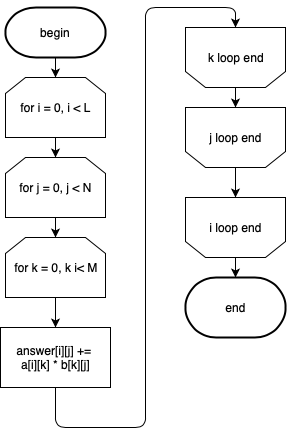
\includegraphics[width=70mm, height=120mm]{multiply.png}
	\caption{Схема стандартного алгоритма\label{overflow}}
\end{figure}
\newpage
\newpage
\begin{figure}[ht!]
	\centering
	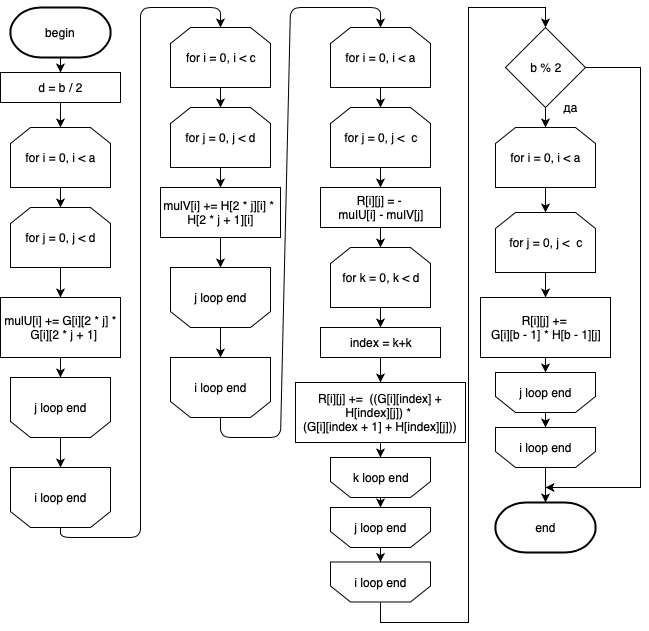
\includegraphics[width=150mm, height=150mm]{opt-2.png}
	\caption{Схема алгоритма улучшенного Винограда \label{overflow}}
\end{figure}

\newpage
\newpage

\section{Технологическая часть}

В этом разделе приведена реализация функций, указан язык программирования и необходимые модули. 
\subsection{Средства реализации}
В данной работе использовался язык Python 3.6, в среде Pycharm. Для измерения времени использовался модуль time, измерения производились в секундах.
Для реализации потоков используется threading, функция Thread которого позволяет создавать потоки. Функция получает на вход имя функции, которая будет реализована в потоке и ее аргументы. 
\subsection{Листинг кода}
\lstset{ 
	backgroundcolor=\color{white},   % choose the background color; you must add \usepackage{color} or \usepackage{xcolor}; should come as last argument
	basicstyle=\footnotesize,        % the size of the fonts that are used for the code
	breakatwhitespace=false,         % sets if automatic breaks should only happen at whitespace
	breaklines=true,                 % sets automatic line breaking
	captionpos=b,                    % sets the caption-position to bottom
	commentstyle=\color{mygreen},    % comment style
	deletekeywords={...},            % if you want to delete keywords from the given language
	escapeinside={\%*}{*)},          % if you want to add LaTeX within your code
	extendedchars=true,              % lets you use non-ASCII characters; for 8-bits encodings only, does not work with UTF-8
	frame=single,	                   % adds a frame around the code
	keepspaces=true,                 % keeps spaces in text, useful for keeping indentation of code (possibly needs columns=flexible)
	keywordstyle=\color{blue},       % keyword style
	language=Python,                 % the language of the code
	morekeywords={*,...},            % if you want to add more keywords to the set
	numbers=left,                    % where to put the line-numbers; possible values are (none, left, right)
	numbersep=5pt,                   % how far the line-numbers are from the code
	numberstyle=\tiny\color{mygray}, % the style that is used for the line-numbers
	rulecolor=\color{black},         % if not set, the frame-color may be changed on line-breaks within not-black text (e.g. comments (green here))
	showspaces=false,                % show spaces everywhere adding particular underscores; it overrides 'showstringspaces'
	showstringspaces=false,          % underline spaces within strings only
	showtabs=false,                  % show tabs within strings adding particular underscores
	stepnumber=1,                    % the step between two line-numbers. If it's 1, each line will be numbered
	stringstyle=\color{mymauve},     % string literal style
	tabsize=1,	                   % sets default tabsize to 2 spaces
	title=Листинг 1. Реализация алгоритмов.                   % show the filename of files included with \lstinputlisting; also try caption instead of title
}
\lstinputlisting[language=Python]{main.py}
\newpage

\newpage
\newpage

\section{Экспериментальная часть}
В данном разделе будут приведены примеры работы алгоритмов и произведены замеры времени. Тестирование производилось на компьютере с процессором Intel Core i5 (I5-6267U) и оперативной памятью 8 Гб. 
\subsection{Примеры работы}
Пример результата работы умножения матриц. Так как в данной реализации генерируются случайные значения, то для проверки результата использовалась библиотека Numpy. При одинаковых входных данных алгоритмы выдают одинаковый результат, который сравнивается с результатом умножния с помощью функции numpy.matmul(). Для вычисления используются квадратные матрицы.
\newline

{\centering
$$\begin{bmatrix} 
12 & 14 & 20 \\
24 & 14 & 16 \\
\end{bmatrix}
+
\begin{bmatrix} 
11 &15\\
8 & 15 \\
14 & 15 \\
\end{bmatrix}
=
\begin{bmatrix} 
524 & 690 \\
600 & 810 \\
\end{bmatrix}$$
}

\subsection{Сравнительный анализ}
Сравнение алгоритмов стандартного умножения и улучшенного алгоритма Винограда в зависимости от количества потоков. На графиках приведены замеры времени работы для матрицы. Каждый экперимент проводился 30 раз, результат - среднее арифметическое замеров времени. 
\newline
\begin{tikzpicture}
\begin{axis}
[
axis x line=middle,
axis y line=middle,
enlarge y limits=true,
xmin=90, xmax=1000,
ymin=0, ymax=375,
width=15cm, height=15cm,     % size of the image
grid = major,
grid style={dashed, gray!30},
ylabel=Время в сек,
xlabel=Размерность матрицы,
legend style={at={(0.1,-0.1)}, anchor=north}
]
\addplot table [x=length, y=basic, col sep=comma] {even.txt};
\addplot table [x=length, y=wino, col sep=comma] {even.txt};
\addplot table [x=length, y=opt, col sep=comma] {even.txt};
\legend {Обычный, Виноград, Улучшеный}
\end{axis}
\end{tikzpicture}
\begin{tikzpicture}
\begin{axis}
[
axis x line=middle,
axis y line=middle,
enlarge y limits=true,
xmin=90, xmax=1002,
ymin=0, ymax=390,
width=15cm, height=15cm,     % size of the image
grid = major,
grid style={dashed, gray!30},
ylabel=Время в сек,
xlabel=Размерность матрицы,
legend style={at={(0.1,-0.1)}, anchor=north}
]
\addplot table [x=length, y=basic, col sep=comma] {uneven.txt};
\addplot table [x=length, y=wino, col sep=comma] {uneven.txt};
\addplot table [x=length, y=opt, col sep=comma] {uneven.txt};
\legend {Обычный, Виноград, Улучшеный}
\end{axis}
\end{tikzpicture}
\newpage
\subsection{Вывод}

\newpage
\section{Заключение}
В лабораторной работе разработаны алгоритмы параллельного вычисления для умножения матриц.  Разработаны программы по этим алгоритмам, проведены тесты по времени, произведен сравнительный анализ алгоритмов. Для составления отчета использован Latex.
\\
\end{document}